\section{Process's Perspective} \label{sec:process}
In this section we present how we organized the development process.

\subsection{The team}
Dudes is a \textit{close-knit team} consisting of five Master students. We value an in-person working environment when possible, which also means that a majority of project work and general interactions have taken place in-person at school during the course hours. With our collective expertise, we have tackled most challenges collaboratively, working together to find solutions. This approach has fostered a seamless workflow, enabling efficient problem-solving and encouraging a sense of shared accomplishment within our team. For work intensive weeks where we did not manage to finish within the course hours, we usually continued on Fridays or Saturdays either at school or remote, but still collaboratively.

\subsection{Version control setup}

Our version control system setup revolves around a monorepo approach, providing a centralized repository to manage our codebase. We have chosen this approach to consolidate all related code in a single repository, promoting the ease of code reuse and streamlining collaboration.
To enhance our workflow and issue tracking, we utilize GitHub's built-in issues extensively. The issues created in GitHub follow predefined templates\footnote{\href{https://github.com/Lindharden/DevOps/tree/main/.github/ISSUE\_TEMPLATE}{github.com/Lindharden/DevOps/tree/main/.github/ISSUE\_TEMPLATE}.}, defined with GitHub issue templates, in order to ensure consistent issue management and to establish guidelines for issue creation, assignment, and resolution. These templates provide a structured framework for issue creation, ensuring all necessary information is captured for the respective type of issue, whether it be bug reports, feature requests, or security vulnerabilities. Additionally, we have implemented a well-defined branching strategy, as shown in figure \ref{fig:branching_flow}, consisting of a main branch as the primary branch, and subbranches designated for the development of single features or bug. The subbranches are named according to a set of naming schemas in order to provide clarity and organization. The naming schemas consists of a predefined tag followed by a relevant name, such as "feature/{feature-name}" or "bug/{bug-name}". Before merging any changes into the main branch, a set of checks is performed to ensure code quality and stability. % These tests includes various types of tests such as unit tests, integration tests, code linting, code formating etc. The purpose of these checks is to catch any potential issues or errors early in the development process, reducing the likelihood of introducing bugs into the main branch. Thus we maintain a higher level of code quality and ensure that the main branch remains stable and functional.
\begin{figure}[H]
    \centering
    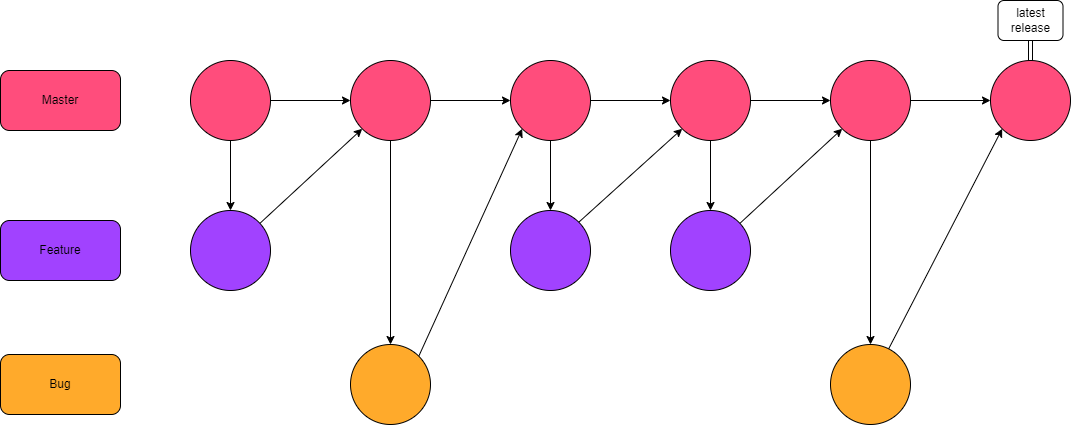
\includegraphics[width=\textwidth]{images/branching_flow.png}
    \caption{Illustration of our GitHub branching flow.}
    \label{fig:branching_flow}
\end{figure}

This branching strategy enables seamless feature development, bug fixing, and code maintenance, ensuring a streamlined development process and promoting collaboration within our team. % (Enables isolated development through clear branching without interfering with one another, parallel development with branching, easy integration with pull requests, clear ownership in order to identify responsibility which facilitates effective communication, and lastly code stability through checks. 
To track releases and provide visibility into the version history, we utilize the GitHub Releases feature. This feature is configured to automatically create a new release for each deployment, ensuring the latest release is always up-to-date with the deployed version. In addition to the automatic releases, we also implemented a weekly release schedule. This manual process allows us to consolidate any significant and relevant features or updates that have been developed during the week. By creating weekly releases, we provide a clear and structured approach to showcasing our progress and informing about the latest developments.


\subsection{CI/CD} \label{sec:cicd}

For our CI/CD setup, we leveraged the capabilities of GitHub Actions to automate the verification process when code is merged into the main branch. GitHub Actions allows us to define custom workflows that encompasses various stages of our pipeline. Within these workflows, we incorporated essential steps to ensure code quality and reliability.

Firstly, the actions execute unit tests to validate the functionality of our codebase, ensuring that it meets the expected behavior. Secondly, we integrated static analysis tools into the workflow, specifically Lint for Go, Snyk, CodeQL, and SonarCloud. These third-party services thoroughly analyze our code to detect potential security vulnerabilities, code smells, and many other potential issues, assisting in maintaining a high level of code quality. 
Lastly, once all the checks pass successfully, GitHub automatically builds a Docker image of our project and deploys it to our hosting service. This ensures that the latest version of the application is available to the users.

To further enhance our development workflow, we integrated GitHub Actions with the pull request feature. This integration enables us to run tests and analysis on proposed changes before merging them into the main branch, minimizing the risk of introducing faulty code into the main branch.

The integration capabilities and the support for automated tests provided by GitHub Actions were key factors in our decisions to choose this CI/CD solution. Our setup streamlines the development process, automates quality checks, and ensures our code is validated and ready for deployment upon introducing changes.

\subsection{Monitoring \& logging}
The monitoring system we have implemented for Minitwit is Prometheus. We have implemented application monitoring and infrastructure monitoring with the following metrics:
\begin{itemize}
    \item \textbf{Number of tweet per hour} - This helps us determine the load our application is under. With this we will be able to see whether the system is overloading or not.
    \item \textbf{Error codes} - This metric shows us the total amount of errors which the system reports. This metric can be used to determine whether everything runs as expected. If the dashboard displays an unusual amount of errors, this might be a hint that something is going on with the system.
    \item \textbf{Response time} - This metric tracks how many milliseconds a user has to wait for a response. This is useful to see if any network issues arise and also to ensure that we uphold the expected average response time of <50ms included in our API SLA.\footnote{\href{https://github.com/Lindharden/DevOps/blob/main/SLA.md}{github.com/Lindharden/DevOps/blob/main/SLA.md}}
    \item \textbf{Hardware load} - This metric reports system load, CPU and memory usage, disk I/O and amount of network transmit and receive requests. This can be useful for determining whether everything runs as expected and whether the hosting server has sufficient resources to handle the incoming load.
\end{itemize}
We use a Grafana dashboard to display the data collected for each metric through Prometheus, which can be seen in figure \ref{fig:grafana_dashboard}. The dashboard is configured through a JSON file\footnote{\href{https://github.com/Lindharden/DevOps/blob/main/monitoring/grafana/dashboards/main.json}{github.com/Lindharden/DevOps/blob/main/monitoring/grafana/dashboards/main.json}.}. Both Prometheus and Grafana have been integrated into the application through the docker-compose.yml configuration file.\footnote{\href{https://github.com/Lindharden/DevOps/blob/main/docker-compose.yml}{github.com/Lindharden/DevOps/blob/main/docker-compose.yml}.}

\begin{figure}[H]
    \centering
    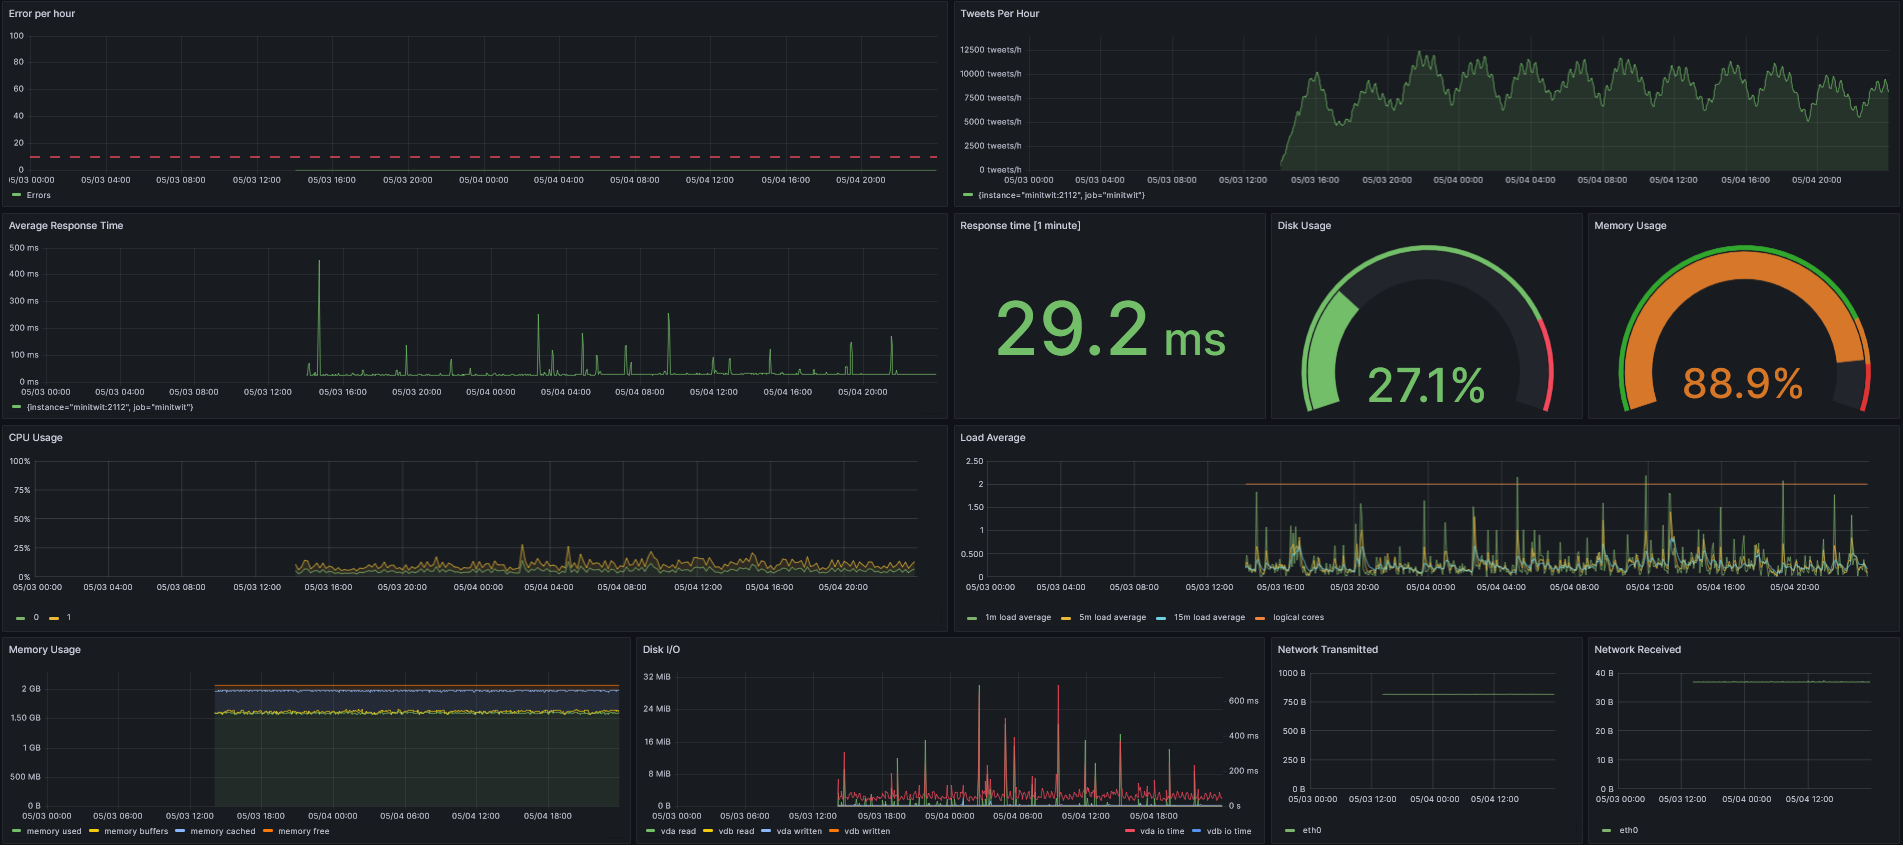
\includegraphics[width=\textwidth]{images/grafana.png}
    \caption{Grafana dashboard displaying the data collected with Prometheus.}
    \label{fig:grafana_dashboard}
\end{figure}

The logging system we have implemented is an EFK stack consisting of Elasticsearch, Filebeat and Kibana. We used the \textit{Zap} package for Go to nicely format and emit log messages that Filebeat collects. We have two types of log messages, the first being the native Ginlog messages that happen for every request. The second one is the log messages that we have implemented in the code, which are formatted by \textit{Zap} in JSON as follows (values are examples):

\begin{figure}[H]
    \begin{footnotesize}
        \begin{minted}{json}
{
   "level":"error",
   "timestamp":"2023-03-25T13:09:38Z",
   "caller":"controllers/loginController.go:130",
   "msg":"Could not find session",
   "user":"John Doe",
   "stacktrace":"..."
}
        \end{minted}
    \end{footnotesize}
    \label{fig:my_label}
\end{figure}

The Kibana dashboard can be seen in figure \ref{fig:kibana_dashboard}. The EFK stack is integrated into the application through the docker-compose.yml configuration file.

\begin{figure}[H]
    \centering
    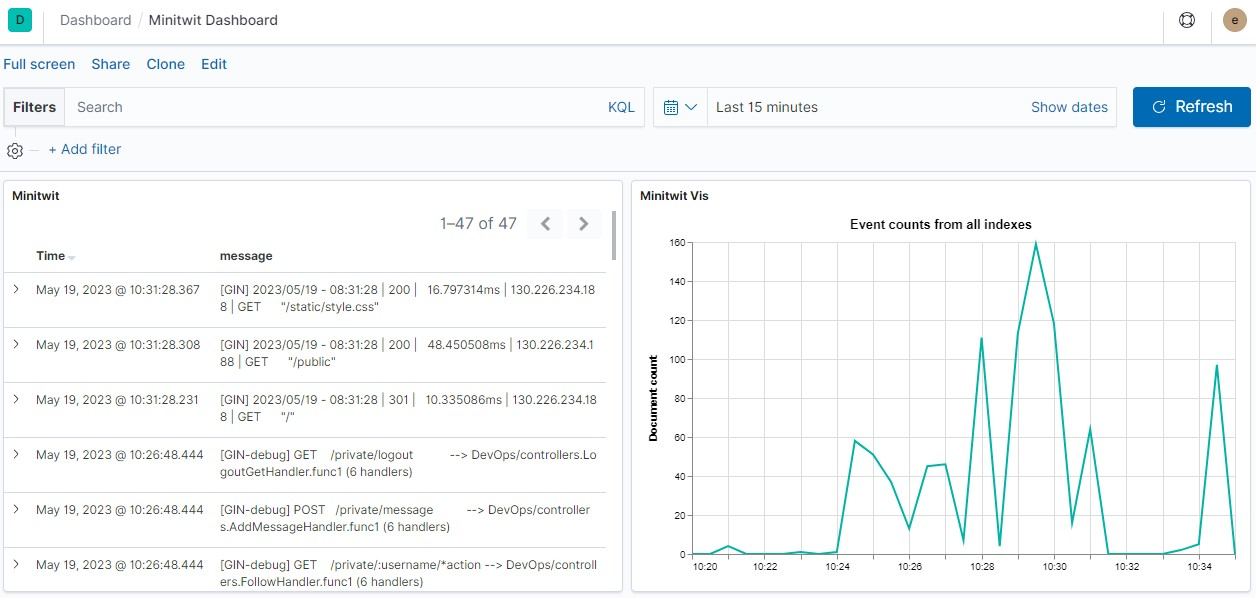
\includegraphics[width=\textwidth]{images/kibana.jpg}
    \caption{Kibana dashboard displaying the logs that are collected, organised and stored by Filebeat and Elastic search.}
    \label{fig:kibana_dashboard}
\end{figure}

\subsection{Security assessment}
In our security assessment we have considered which risks the infrastructure and application are vulnerable to. The risks we have assessed are mapped in a risk assessment matrix which can be seen in figure \ref{fig:risk_matrix}. More concretely they are:
\begin{itemize}
    \item \textbf{Compromised GitHub repository} - The GitHub repository owner uses two-factor authentication. Furthermore, all users must make a pull request and have it approved to change the code on the main branch. This makes it unlikely that the GitHub repository is compromised. However, a compromised GitHub repository would mean that the attacker would gain access to one of our GitHub admin accounts, which would mean they have the ability to change our code, making it a significant impact risk.
    \item \textbf{White-box exploits} - As our GitHub repository is public, anyone can see our code and create exploits for it. Therefore if the attacker finds a reason and an opportunity to create a white-box exploit, it would likely happen. However, as we continuously update our code and update vulnerable packages, the chance of an exploit being possible is very low. As the attacker knows what our code base looks like they can plan their attacks towards having as large of an impact as possible. In addition, the attacker can see all the dependencies we use, meaning they can utilize any exploits found in our dependencies, making it an extensive impact risk.
    \item \textbf{DDoS attack} - Since our application is not that popular it is not likely that it will get DDoS’ed, but it is still possible since our application is public. A DDoS attack would mean that our application would be unreachable for a period of time. This would be a moderate inconvenience for us and our users, making it a moderate impact risk.
    \item \textbf{SQL injection} - Since our database abstraction layer GORM sanitizes all keywords, an SQL injection attack is very rare, basically impossible. SQL injection would mean that an attacker performs attacks directly on our database, by sending arbitrary SQL queries, making it an extensive impact risk.
    \item \textbf{DB leak} - The only ways our database can be leaked, is by someone compromising our code repository and performing some kind of white-box exploit, or by performing SQL injection. As we deemed these risks as “rare”, our database leaking must also be a rare event. If our database leaked, the attacker would gain access to usernames, email’s and hashed passwords of our users. As none of this is sensitive information the impact would be negligible.
\end{itemize}

\begin{figure}[H]
    \centering
    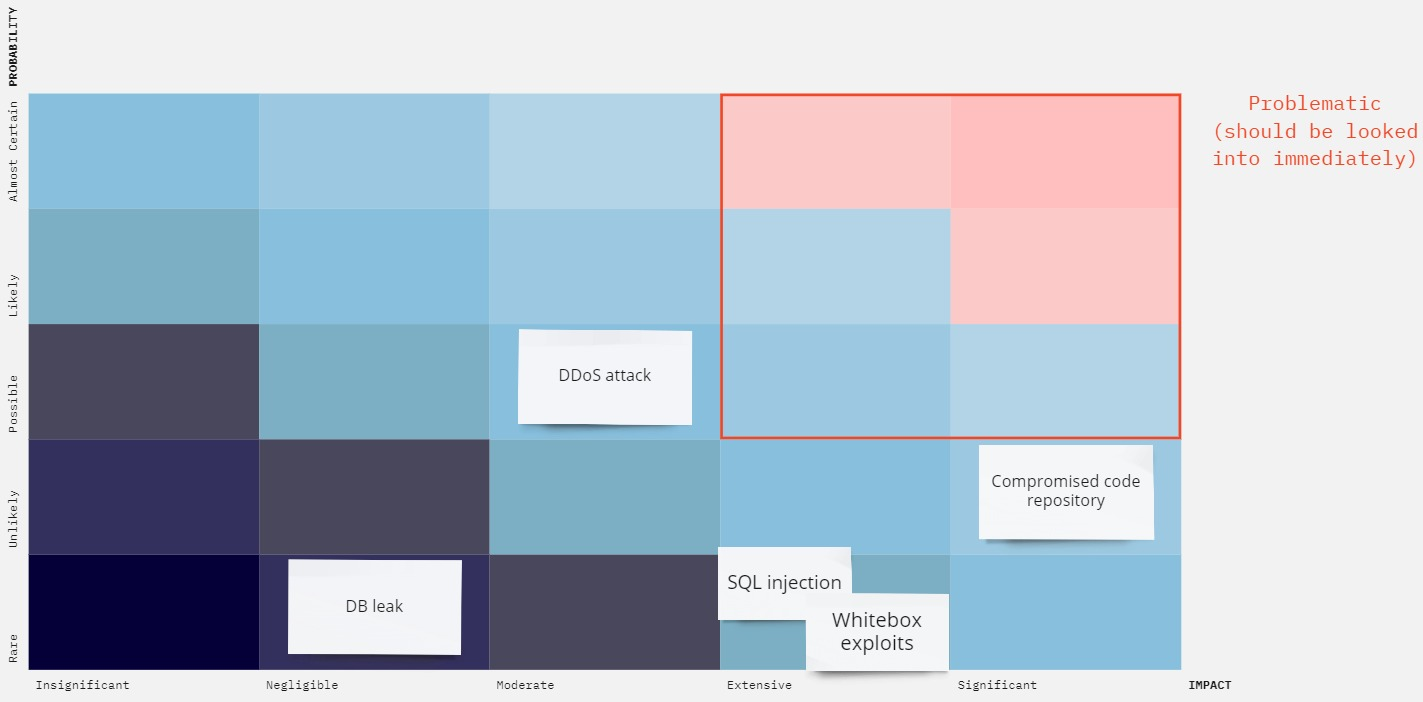
\includegraphics[width=\textwidth]{images/risk_matrix.png}
    \caption{Risk assessment matrix. The vertical axis indicates the probability of a risk while the horizontal axis indicates the impact of a risk. Risks in the top-right corner are considered problematic and should be handled accordingly.}
    \label{fig:risk_matrix}
\end{figure}

None of the assessed risks are placed inside the problematic area in the risk assessment matrix in figure \ref{fig:risk_matrix}. Therefore, we have not taken any actions against these risks, we have simply decided to accept them for now. Additionally, we generated a vulnerability report using Zap which can be found here: \href{https://htmlpreview.github.io/?https://github.com/Lindharden/DevOps/blob/main/docs/OWASP_ZAP/report_290323/2023-03-29-ZAP-Report-.html}{github.com/Lindharden/DevOps/blob/main/docs/OWASP\_ZAP/report\_290323/2023-03-29-ZAP-Report-.html}. This report didn't show any major vulnerabilities.

\subsection{Scaling \& redundancy} \label{sec:scaling}
To ensure fault tolerance we introduced redundancy in the form of a replica. We created an additional droplet on DigitalOcean and changed our Vagrantfile accordingly to have identical instances running on each of the droplets. One of the instances act as the primary one, for which all traffic is directed to. The other instance serves as a backup. With the use of heartbeats the server can keep track of the primary replicas state, and should it fail to show signs of life, the backup replica will take over as primary.

In addition to fault tolerance, having a primary and backup replica also enables rolling updates which eliminates the inevitable downtime caused from deploying updates. We did not get around to do it for this project, but we had a plan of how we wanted to do it. In order to increase our availability, we will first be updating the backup replica and make it our primary server, then we can shut down the replica which was previously the primary one and update it as well. We facilitate this process by using DigitalOcean's API to automatically switch the primary server to the running replica.